
\section{Robustness checks and implementation details for the simulations in Section \ref{sec-sim}}\label{sec-supp-sim}


\subsection*{Robustness checks for Section \ref{subsec-sim-3}}


In what follows, we carry out some robustness checks to assess how sensitive the estimators $\widehat{a}$ and $\widehat{\sigma}^2$ are to the choice of the tuning parameters $q$ and $(\underline{r},\overline{r})$. To do so, we repeat the simulation exercises of Section \ref{subsec-sim-3} for different values of $q$ and $(\underline{r},\overline{r})$. In addition, we consider different choices of the tuning parameters $(m_1,m_2)$ on which the estimators of \cite{Hall2003} depend. As in Section \ref{subsec-sim-3}, we choose $m_1$ and $m_2$ such that $q$ lies between these values. We thus keep the parameters $q$ and $(m_1,m_2)$ roughly comparable. We restrict attention to the sample size $T=500$ as the results for $T=250$ lead to essentially the same conclusions. 


To start with, we consider the simulation scenarios with a moderate trend ($s_\beta = 1$). The MSE values of the estimators $\widehat{a}$, $\widehat{a}_{\text{HvK}}$, $\widehat{a}_{\text{oracle}}$ and $\widehat{\sigma}^2$, $\widehat{\sigma}^2_{\text{HvK}}$, $\widehat{\sigma}^2_{\text{oracle}}$ for these scenarios are presented in Figure \ref{fig:MSE_slope1} of Section \ref{subsec-sim-3}. These MSEs are re-calculated in Figures \ref{fig:MSE_slope1_AR_robust} and \ref{fig:MSE_slope1_lrv_robust} for a range of different choices of $q$, $(\underline{r},\overline{r})$ and $(m_1,m_2)$. As one can see, the MSEs in the different plots of Figures \ref{fig:MSE_slope1_AR_robust} and \ref{fig:MSE_slope1_lrv_robust} are very similar. Hence, the MSE results reported in Section \ref{subsec-sim-3} for the scenarios with a moderate trend appear to be fairly robust to different choices of the tuning parameters. In particular, our estimators $\widehat{a}$ and $\widehat{\sigma}^2$ seem to be quite insensitive to the choice of tuning parameters, at least as far as their MSEs are concerned.


We next turn to the simulation designs with a pronounced trend ($s_\beta = 10$). The MSE values of the estimators in these scenarios are reported in Figure \ref{fig:MSE_slope10} of Section \ref{subsec-sim-3}. Analogously as before, we re-calculate these MSEs for different tuning parameters in Figures \ref{fig:MSE_slope10_AR_robust}--\ref{fig:MSE_slope10_lrv_robust}. Figure \ref{fig:MSE_slope10_AR_zoom_robust} is a zoomed-in version of Figure \ref{fig:MSE_slope10_AR_robust} which is added for better visibility. As can be seen, our estimators appear to be barely influenced by the choice of $q$. However, the MSE values become somewhat larger when $\overline{r}$ is chosen bigger. This is of course not very suprising: The main reason why the estimator $\widehat{a}$ works well in the presence of a strong trend is that it is only based on differences of small orders. If we increase $\overline{r}$, we use larger differences to compute $\widehat{a}$ which results in not eliminating the trend $m$ appropriately any more. This becomes visible in somewhat larger MSE values. Nevertheless, our estimators appear not to be strongly influenced by the choice of tuning parameters (in terms of MSE) as long as these are chosen within reasonable bounds. 


\begin{figure}[p]
\begin{subfigure}[b]{0.45\textwidth}
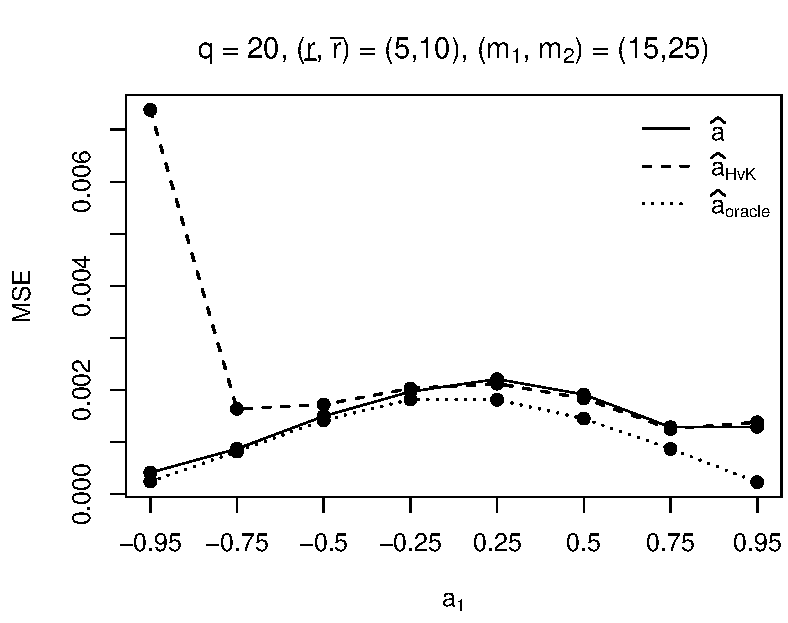
\includegraphics[width=\textwidth]{Plots/Plots_Supplement/MSE_a_T=500_slope=1_(L1,L2,K1,K2,M1,M2)=(20,20,5,10,15,25).pdf}
\end{subfigure}
\hspace{0.25cm}
\begin{subfigure}[b]{0.45\textwidth}
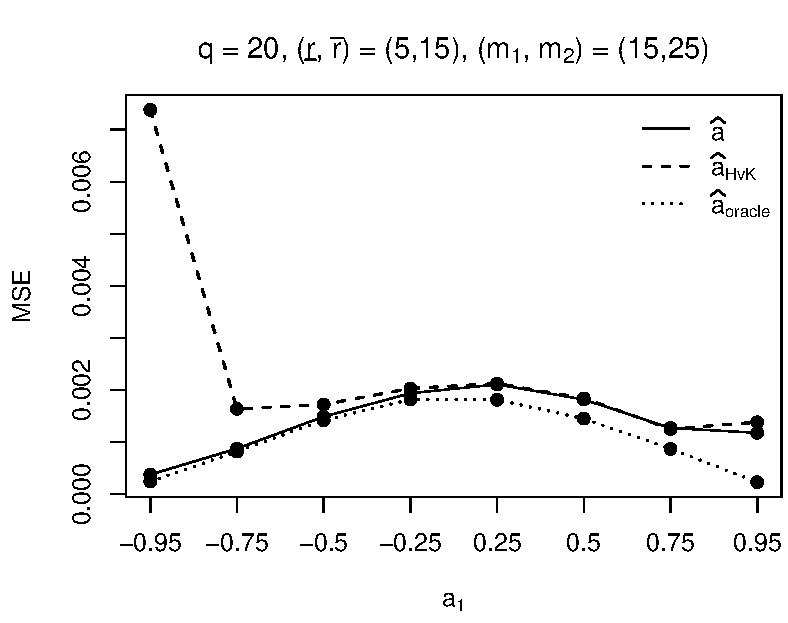
\includegraphics[width=\textwidth]{Plots/Plots_Supplement/MSE_a_T=500_slope=1_(L1,L2,K1,K2,M1,M2)=(20,20,5,15,15,25).pdf}
\end{subfigure}

\begin{subfigure}[b]{0.45\textwidth}
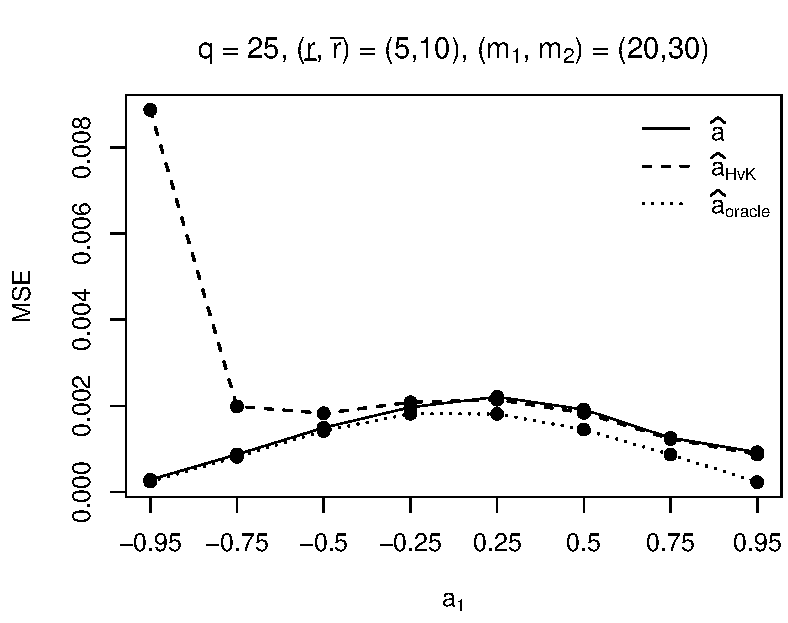
\includegraphics[width=\textwidth]{Plots/Plots_Supplement/MSE_a_T=500_slope=1_(L1,L2,K1,K2,M1,M2)=(25,25,5,10,20,30).pdf}
\end{subfigure}
\hspace{0.25cm}
\begin{subfigure}[b]{0.45\textwidth}
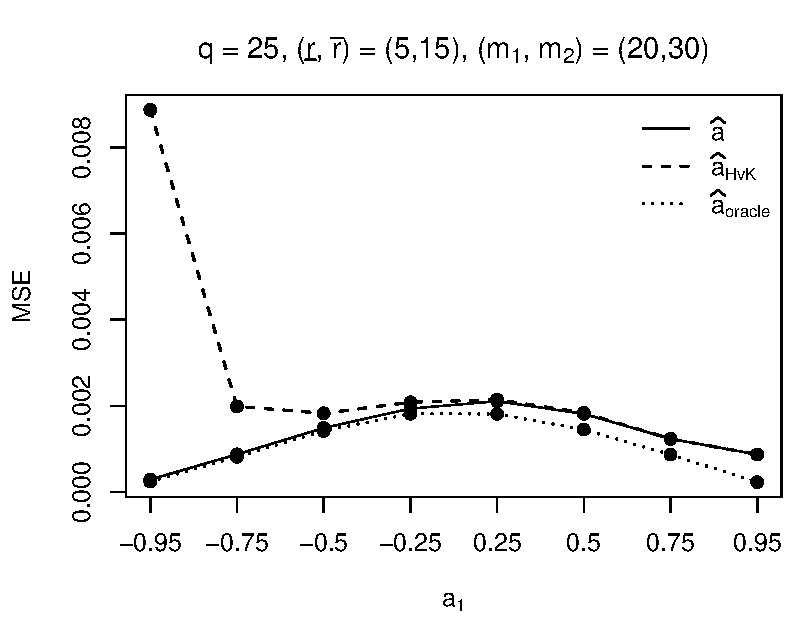
\includegraphics[width=\textwidth]{Plots/Plots_Supplement/MSE_a_T=500_slope=1_(L1,L2,K1,K2,M1,M2)=(25,25,5,15,20,30).pdf}
\end{subfigure}

\begin{subfigure}[b]{0.45\textwidth}
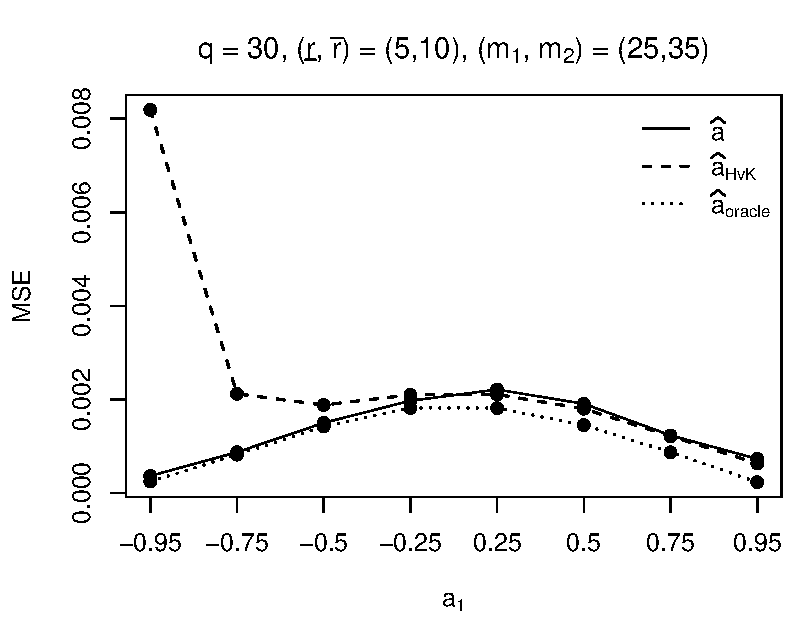
\includegraphics[width=\textwidth]{Plots/Plots_Supplement/MSE_a_T=500_slope=1_(L1,L2,K1,K2,M1,M2)=(30,30,5,10,25,35).pdf}
\end{subfigure}
\hspace{0.25cm}
\begin{subfigure}[b]{0.45\textwidth}
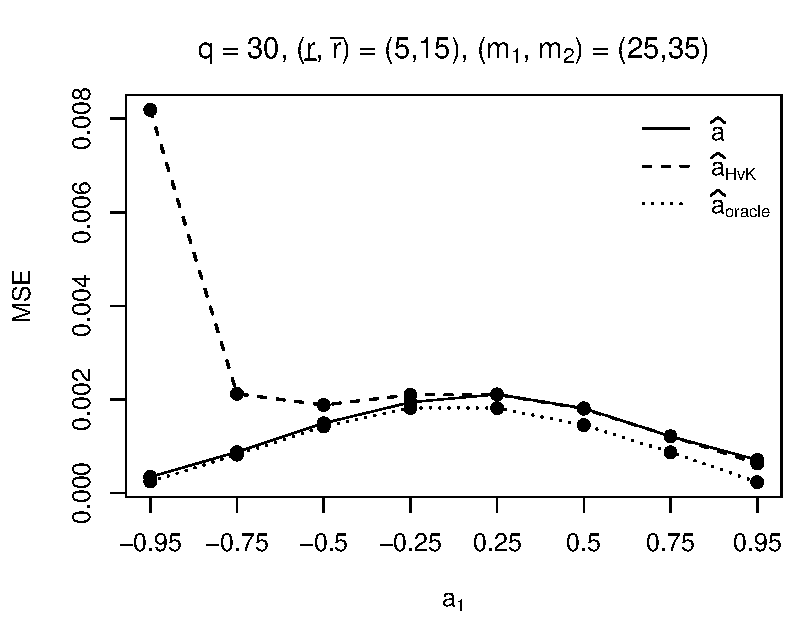
\includegraphics[width=\textwidth]{Plots/Plots_Supplement/MSE_a_T=500_slope=1_(L1,L2,K1,K2,M1,M2)=(30,30,5,15,25,35).pdf}
\end{subfigure}

\begin{subfigure}[b]{0.45\textwidth}
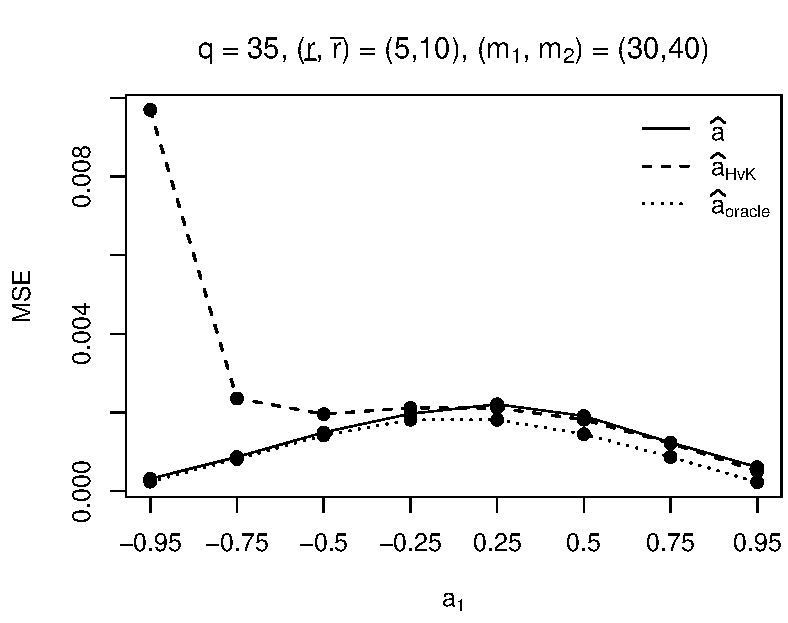
\includegraphics[width=\textwidth]{Plots/Plots_Supplement/MSE_a_T=500_slope=1_(L1,L2,K1,K2,M1,M2)=(35,35,5,10,30,40).pdf}
\end{subfigure}
\hspace{0.25cm}
\begin{subfigure}[b]{0.45\textwidth}
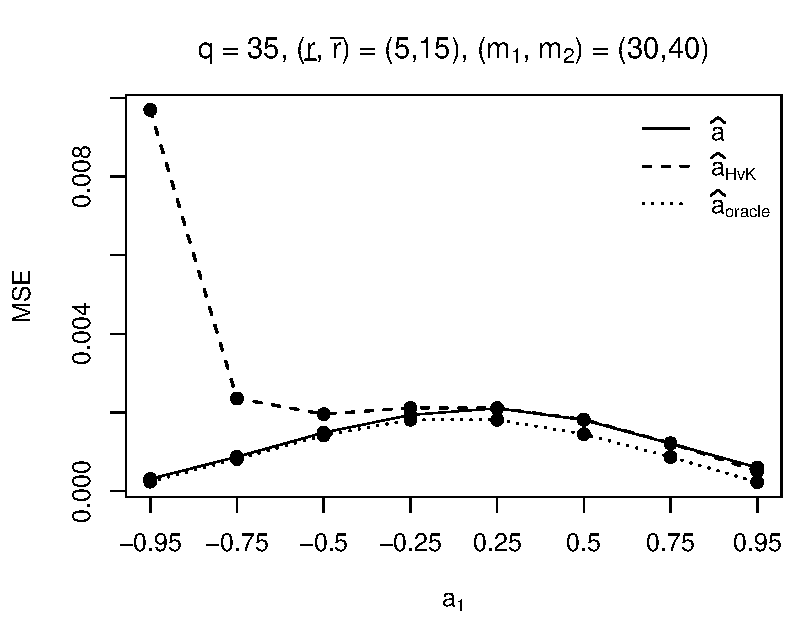
\includegraphics[width=\textwidth]{Plots/Plots_Supplement/MSE_a_T=500_slope=1_(L1,L2,K1,K2,M1,M2)=(35,35,5,15,30,40).pdf}
\end{subfigure}
\caption{MSE values for the estimators $\widehat{a}$, $\widehat{a}_{\text{HvK}}$ and $\widehat{a}_{\text{oracle}}$ in the scenario with $T=500$ and $s_\beta=1$.}\label{fig:MSE_slope1_AR_robust} 
\end{figure}


\begin{figure}[p]
\begin{subfigure}[b]{0.45\textwidth}
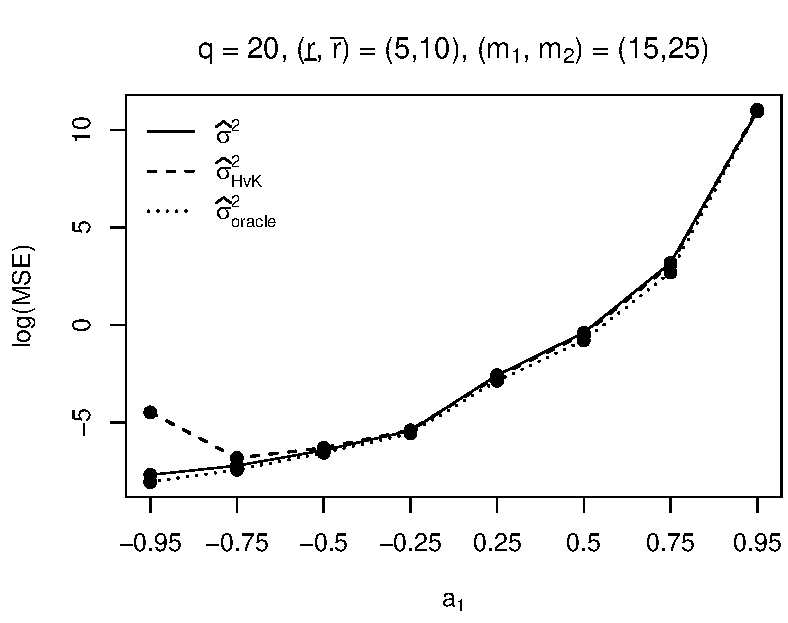
\includegraphics[width=\textwidth]{Plots/Plots_Supplement/MSE_lrv_T=500_slope=1_(L1,L2,K1,K2,M1,M2)=(20,20,5,10,15,25).pdf}
\end{subfigure}
\hspace{0.25cm}
\begin{subfigure}[b]{0.45\textwidth}
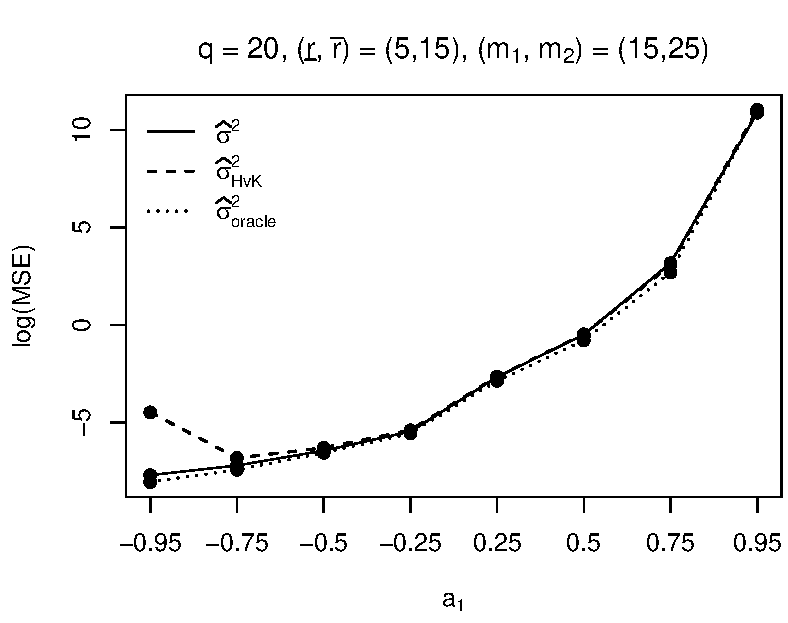
\includegraphics[width=\textwidth]{Plots/Plots_Supplement/MSE_lrv_T=500_slope=1_(L1,L2,K1,K2,M1,M2)=(20,20,5,15,15,25).pdf}
\end{subfigure}

\begin{subfigure}[b]{0.45\textwidth}
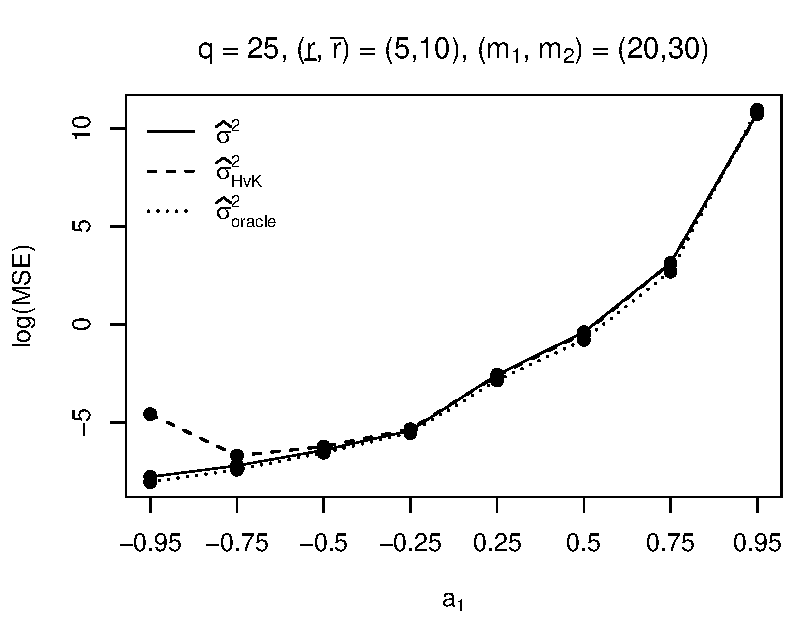
\includegraphics[width=\textwidth]{Plots/Plots_Supplement/MSE_lrv_T=500_slope=1_(L1,L2,K1,K2,M1,M2)=(25,25,5,10,20,30).pdf}
\end{subfigure}
\hspace{0.25cm}
\begin{subfigure}[b]{0.45\textwidth}
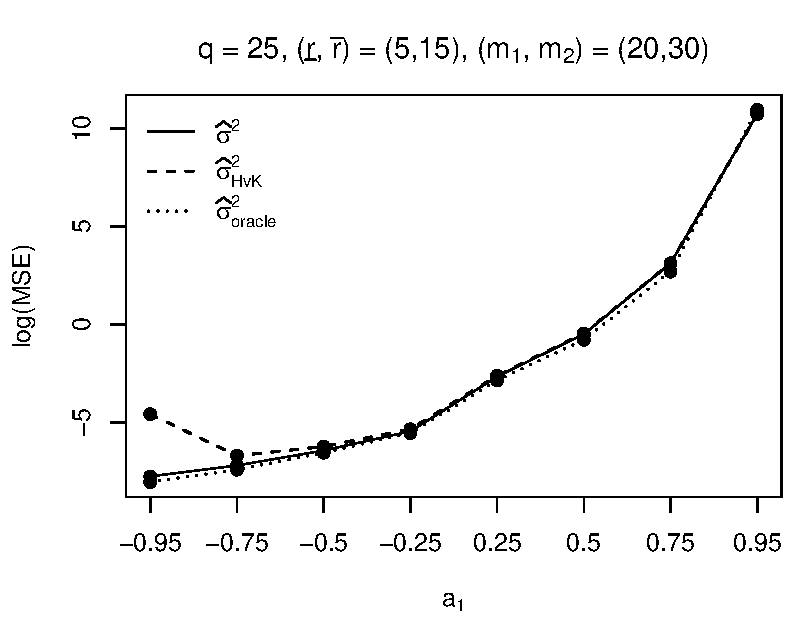
\includegraphics[width=\textwidth]{Plots/Plots_Supplement/MSE_lrv_T=500_slope=1_(L1,L2,K1,K2,M1,M2)=(25,25,5,15,20,30).pdf}
\end{subfigure}

\begin{subfigure}[b]{0.45\textwidth}
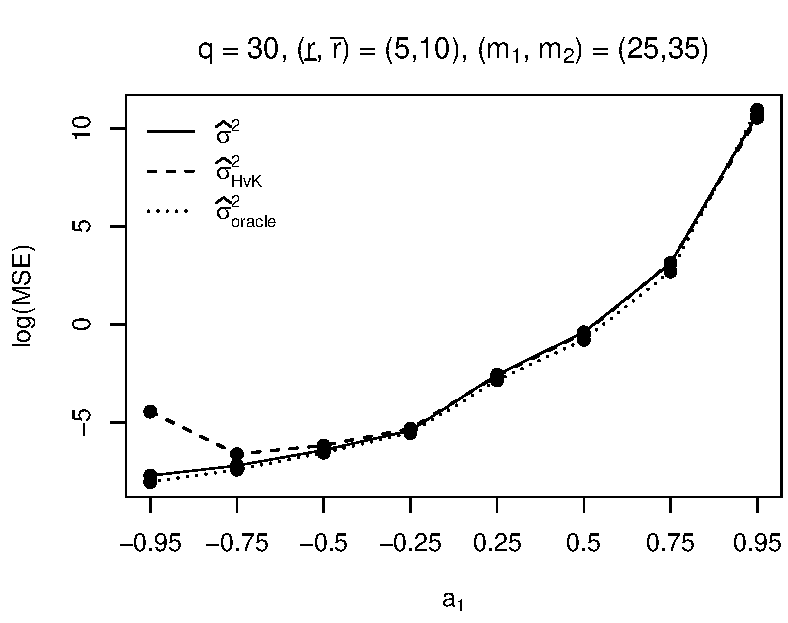
\includegraphics[width=\textwidth]{Plots/Plots_Supplement/MSE_lrv_T=500_slope=1_(L1,L2,K1,K2,M1,M2)=(30,30,5,10,25,35).pdf}
\end{subfigure}
\hspace{0.25cm}
\begin{subfigure}[b]{0.45\textwidth}
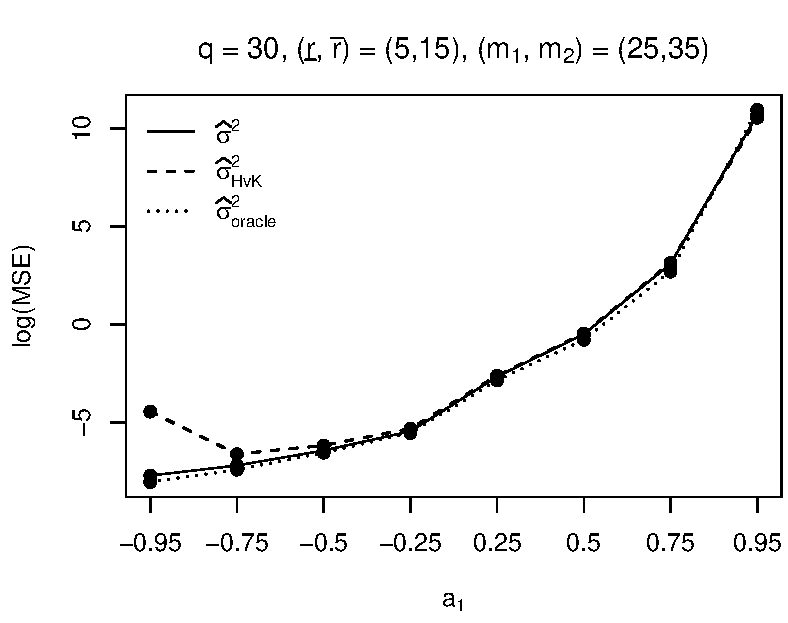
\includegraphics[width=\textwidth]{Plots/Plots_Supplement/MSE_lrv_T=500_slope=1_(L1,L2,K1,K2,M1,M2)=(30,30,5,15,25,35).pdf}
\end{subfigure}

\begin{subfigure}[b]{0.45\textwidth}
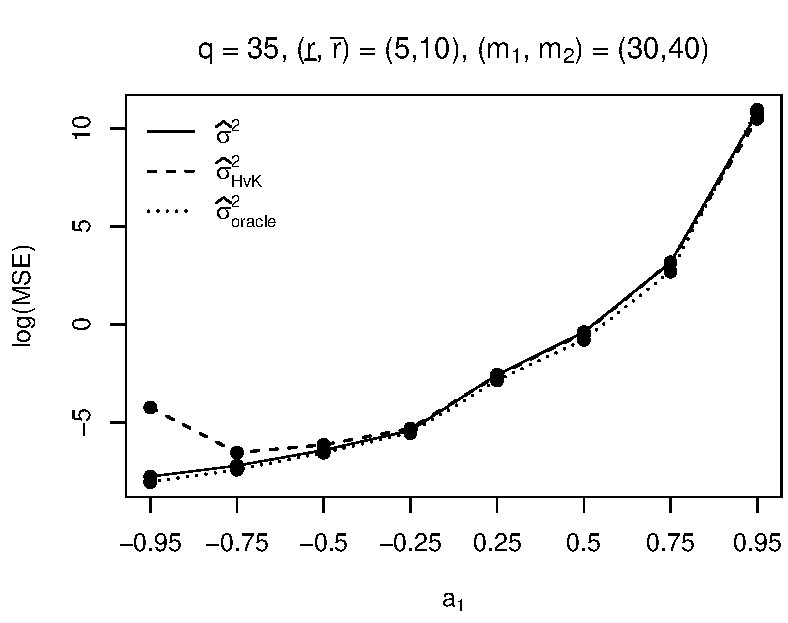
\includegraphics[width=\textwidth]{Plots/Plots_Supplement/MSE_lrv_T=500_slope=1_(L1,L2,K1,K2,M1,M2)=(35,35,5,10,30,40).pdf}
\end{subfigure}
\hspace{0.25cm}
\begin{subfigure}[b]{0.45\textwidth}
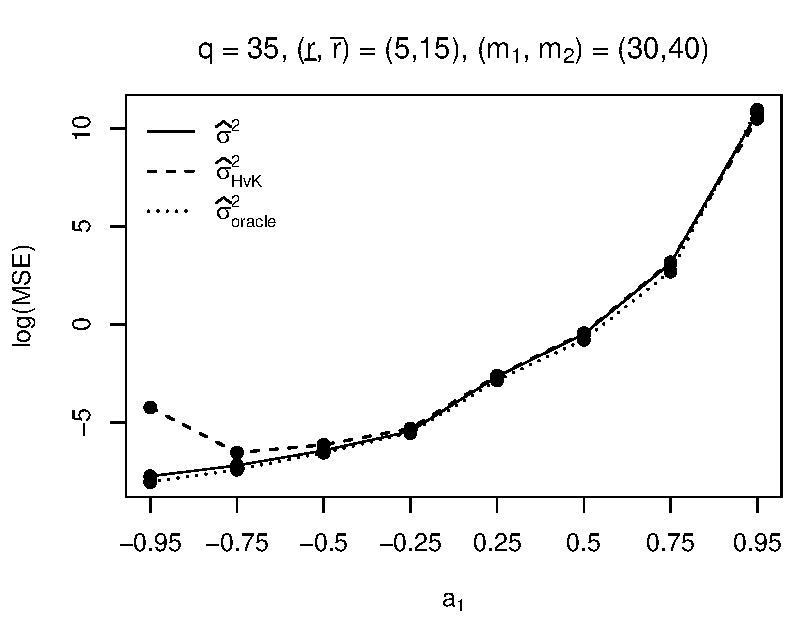
\includegraphics[width=\textwidth]{Plots/Plots_Supplement/MSE_lrv_T=500_slope=1_(L1,L2,K1,K2,M1,M2)=(35,35,5,15,30,40).pdf}
\end{subfigure}
\caption{Logarithmic MSE values for the estimators $\widehat{\sigma}^2$, $\widehat{\sigma}^2_{\text{HvK}}$ and $\widehat{\sigma}^2_{\text{oracle}}$ in the scenario with $T=500$ and $s_\beta=1$.}\label{fig:MSE_slope1_lrv_robust}
\end{figure}


\begin{figure}[p]
\begin{subfigure}[b]{0.45\textwidth}
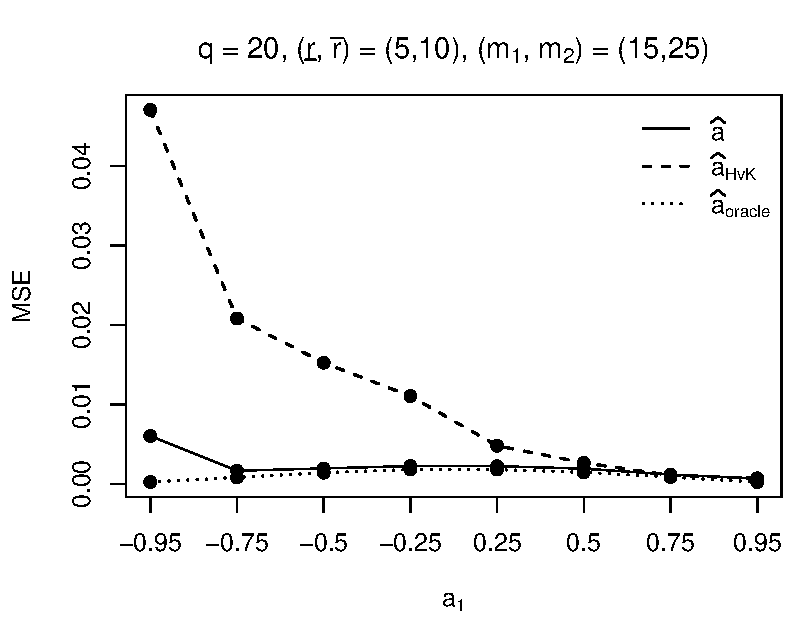
\includegraphics[width=\textwidth]{Plots/Plots_Supplement/MSE_a_T=500_slope=10_(L1,L2,K1,K2,M1,M2)=(20,20,5,10,15,25).pdf}
\end{subfigure}
\hspace{0.25cm}
\begin{subfigure}[b]{0.45\textwidth}
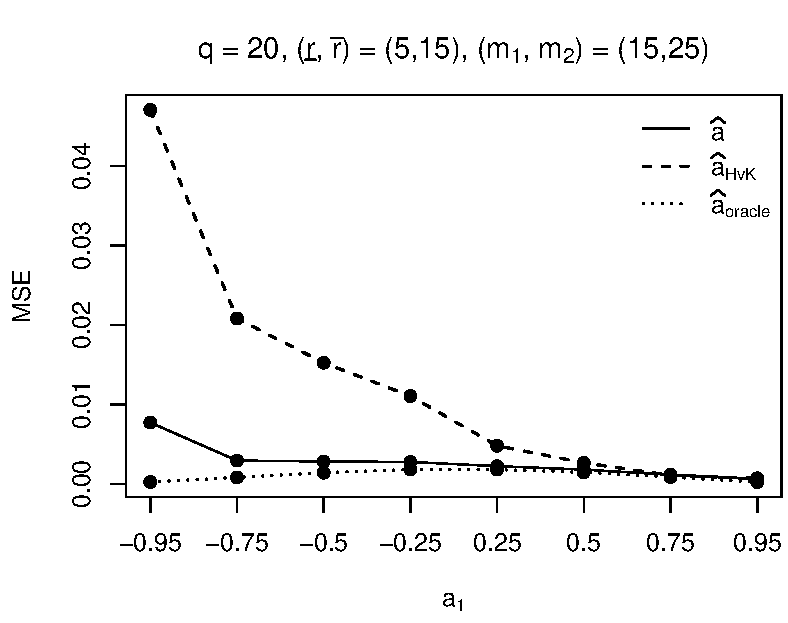
\includegraphics[width=\textwidth]{Plots/Plots_Supplement/MSE_a_T=500_slope=10_(L1,L2,K1,K2,M1,M2)=(20,20,5,15,15,25).pdf}
\end{subfigure}

\begin{subfigure}[b]{0.45\textwidth}
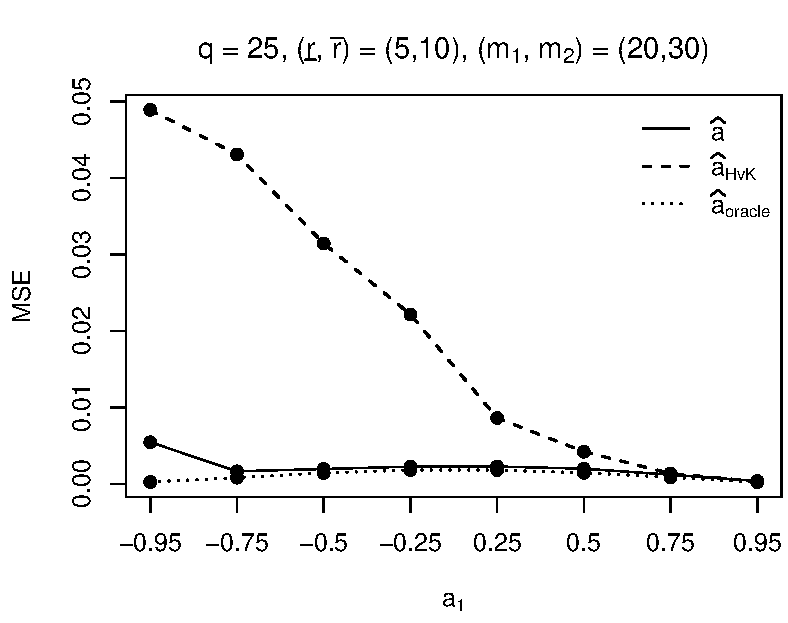
\includegraphics[width=\textwidth]{Plots/Plots_Supplement/MSE_a_T=500_slope=10_(L1,L2,K1,K2,M1,M2)=(25,25,5,10,20,30).pdf}
\end{subfigure}
\hspace{0.25cm}
\begin{subfigure}[b]{0.45\textwidth}
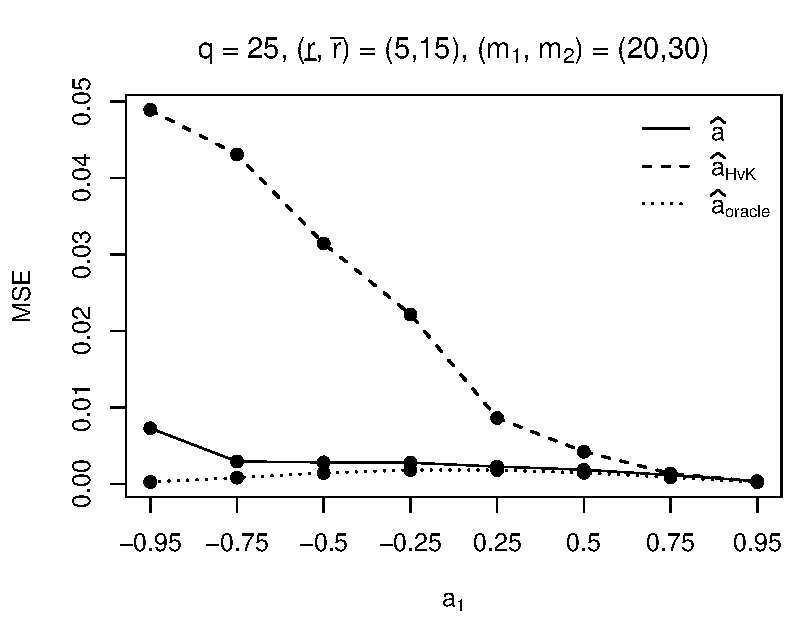
\includegraphics[width=\textwidth]{Plots/Plots_Supplement/MSE_a_T=500_slope=10_(L1,L2,K1,K2,M1,M2)=(25,25,5,15,20,30).pdf}
\end{subfigure}

\begin{subfigure}[b]{0.45\textwidth}
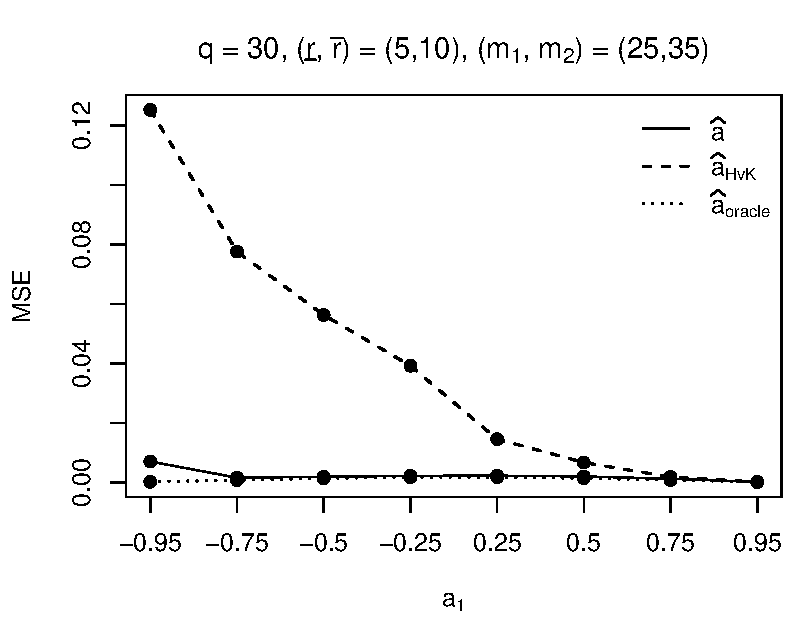
\includegraphics[width=\textwidth]{Plots/Plots_Supplement/MSE_a_T=500_slope=10_(L1,L2,K1,K2,M1,M2)=(30,30,5,10,25,35).pdf}
\end{subfigure}
\hspace{0.25cm}
\begin{subfigure}[b]{0.45\textwidth}
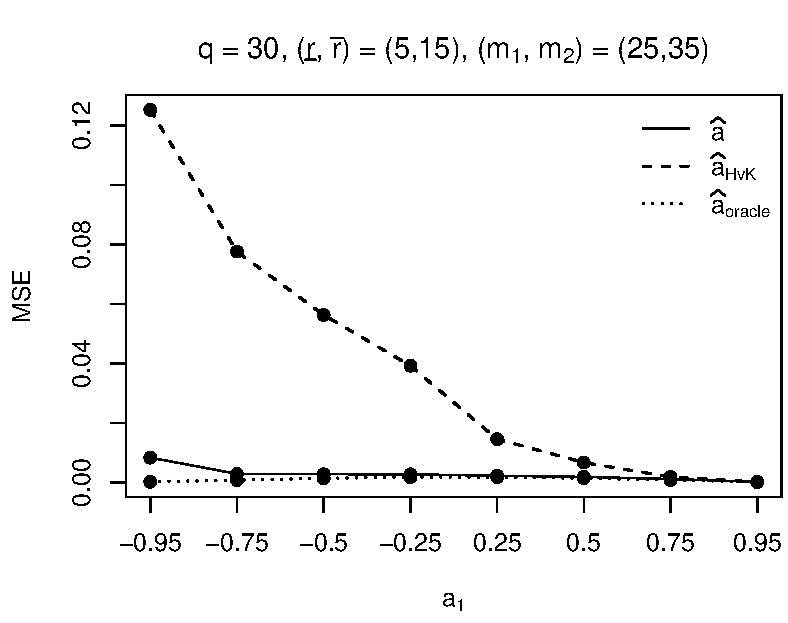
\includegraphics[width=\textwidth]{Plots/Plots_Supplement/MSE_a_T=500_slope=10_(L1,L2,K1,K2,M1,M2)=(30,30,5,15,25,35).pdf}
\end{subfigure}

\begin{subfigure}[b]{0.45\textwidth}
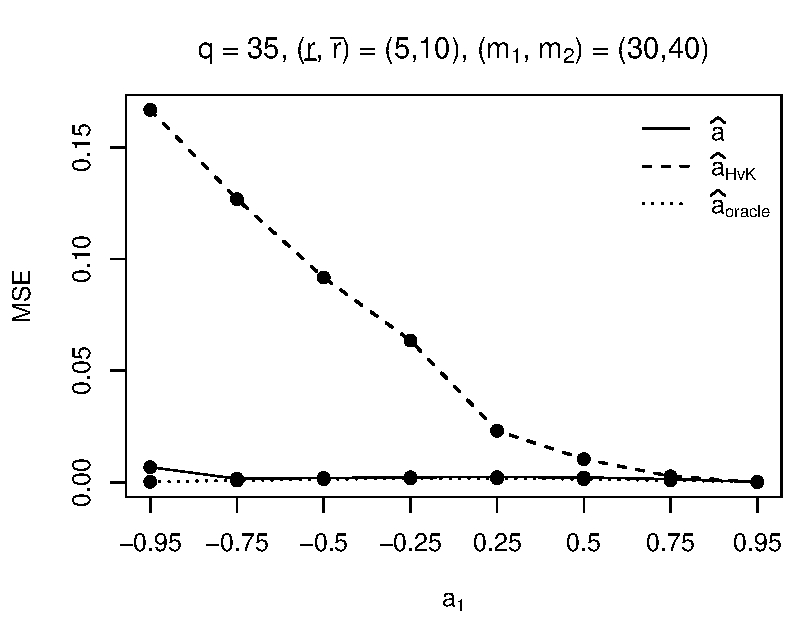
\includegraphics[width=\textwidth]{Plots/Plots_Supplement/MSE_a_T=500_slope=10_(L1,L2,K1,K2,M1,M2)=(35,35,5,10,30,40).pdf}
\end{subfigure}
\hspace{0.25cm}
\begin{subfigure}[b]{0.45\textwidth}
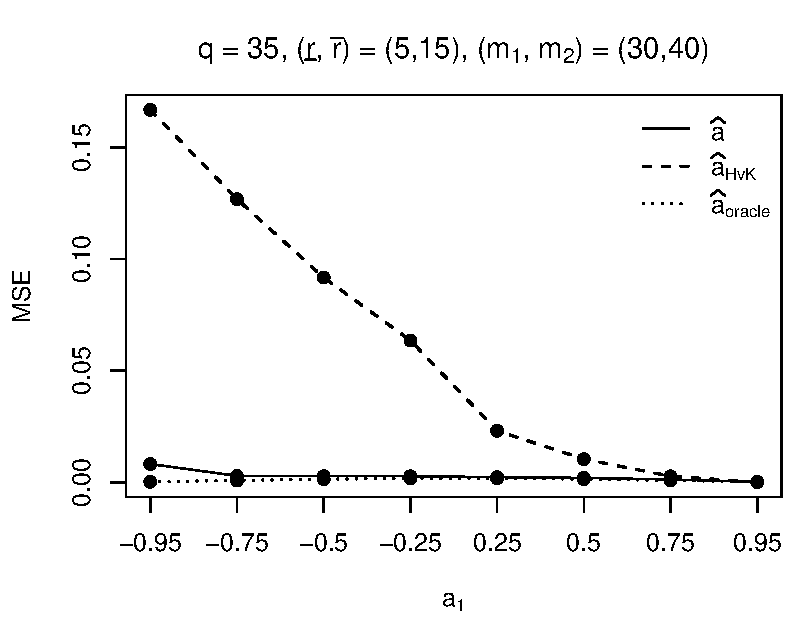
\includegraphics[width=\textwidth]{Plots/Plots_Supplement/MSE_a_T=500_slope=10_(L1,L2,K1,K2,M1,M2)=(35,35,5,15,30,40).pdf}
\end{subfigure}
\caption{MSE values for the estimators $\widehat{a}$, $\widehat{a}_{\text{HvK}}$ and $\widehat{a}_{\text{oracle}}$ in the scenario with $T=500$ and $s_\beta=10$.}\label{fig:MSE_slope10_AR_robust} 
\end{figure}


\begin{figure}[p]
\begin{subfigure}[b]{0.45\textwidth}
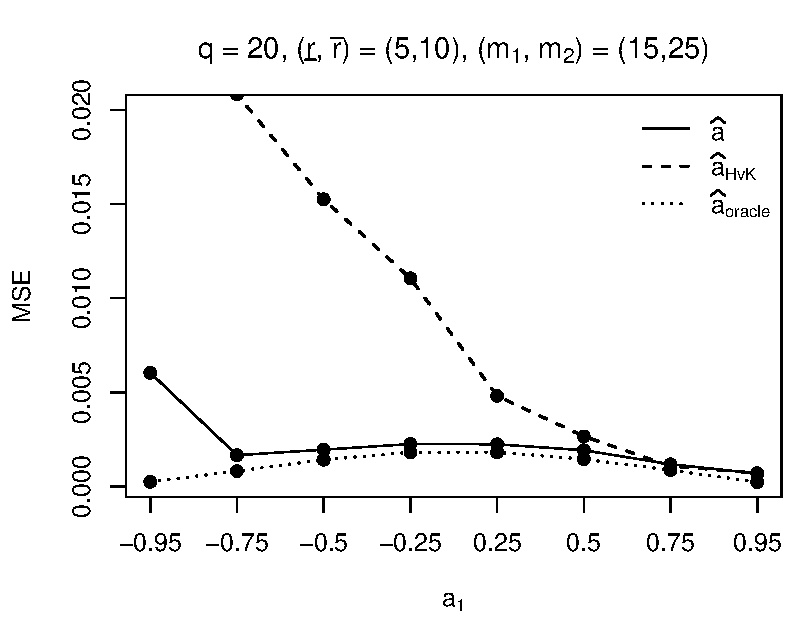
\includegraphics[width=\textwidth]{Plots/Plots_Supplement/MSE_a_zoom_T=500_slope=10_(L1,L2,K1,K2,M1,M2)=(20,20,5,10,15,25).pdf}
\end{subfigure}
\hspace{0.25cm}
\begin{subfigure}[b]{0.45\textwidth}
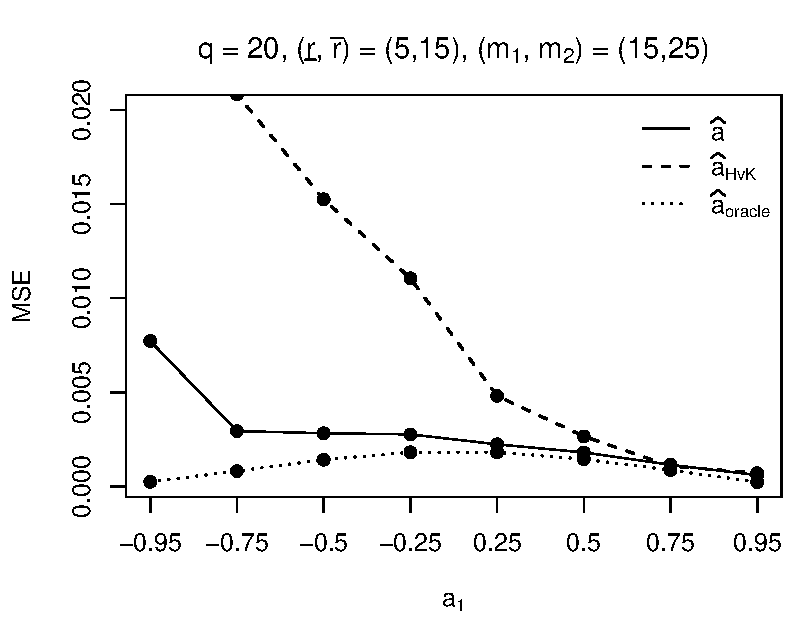
\includegraphics[width=\textwidth]{Plots/Plots_Supplement/MSE_a_zoom_T=500_slope=10_(L1,L2,K1,K2,M1,M2)=(20,20,5,15,15,25).pdf}
\end{subfigure}

\begin{subfigure}[b]{0.45\textwidth}
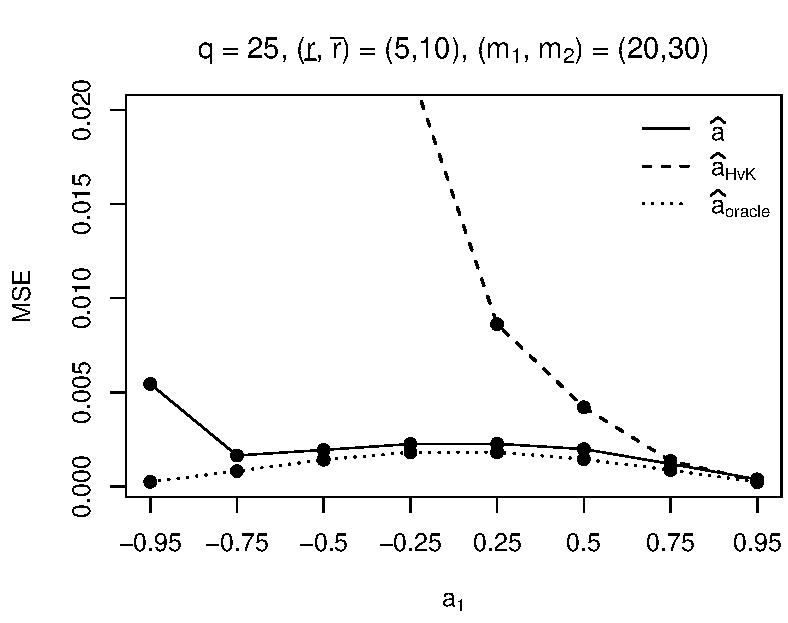
\includegraphics[width=\textwidth]{Plots/Plots_Supplement/MSE_a_zoom_T=500_slope=10_(L1,L2,K1,K2,M1,M2)=(25,25,5,10,20,30).pdf}
\end{subfigure}
\hspace{0.25cm}
\begin{subfigure}[b]{0.45\textwidth}
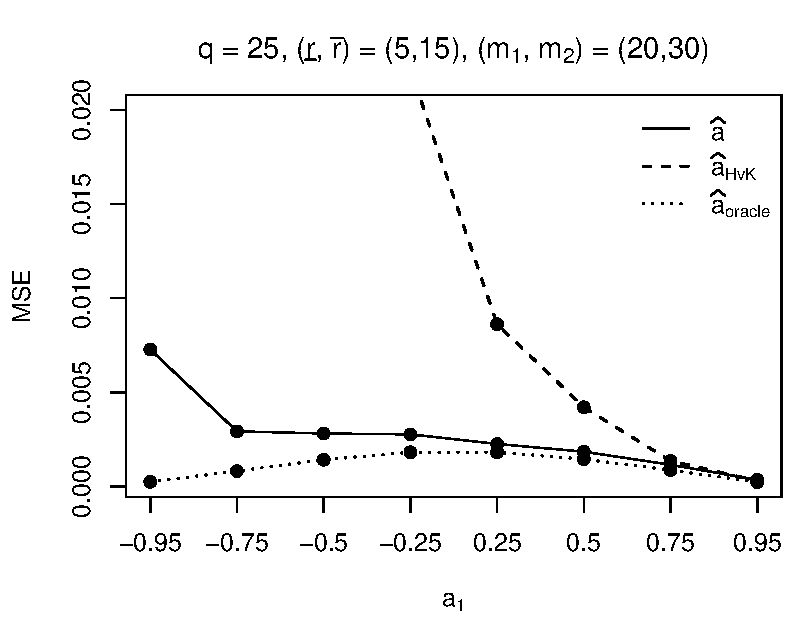
\includegraphics[width=\textwidth]{Plots/Plots_Supplement/MSE_a_zoom_T=500_slope=10_(L1,L2,K1,K2,M1,M2)=(25,25,5,15,20,30).pdf}
\end{subfigure}

\begin{subfigure}[b]{0.45\textwidth}
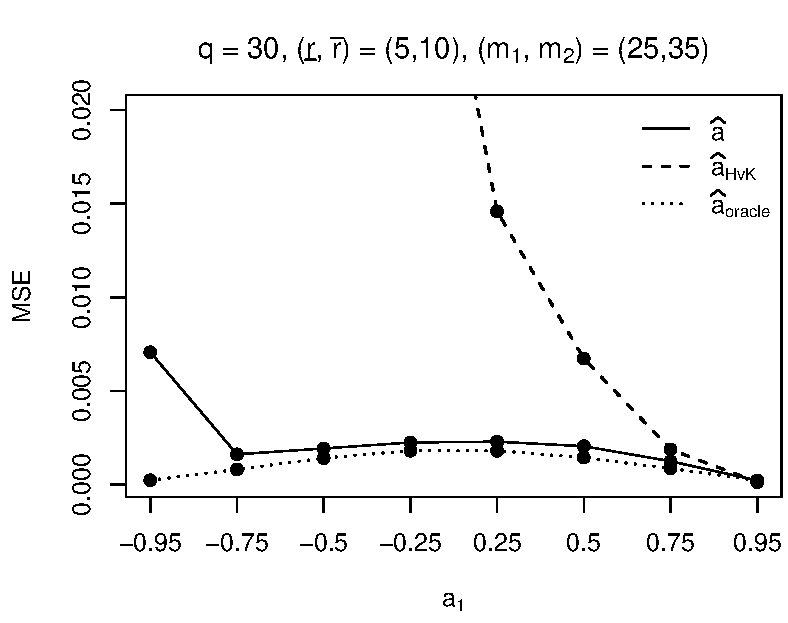
\includegraphics[width=\textwidth]{Plots/Plots_Supplement/MSE_a_zoom_T=500_slope=10_(L1,L2,K1,K2,M1,M2)=(30,30,5,10,25,35).pdf}
\end{subfigure}
\hspace{0.25cm}
\begin{subfigure}[b]{0.45\textwidth}
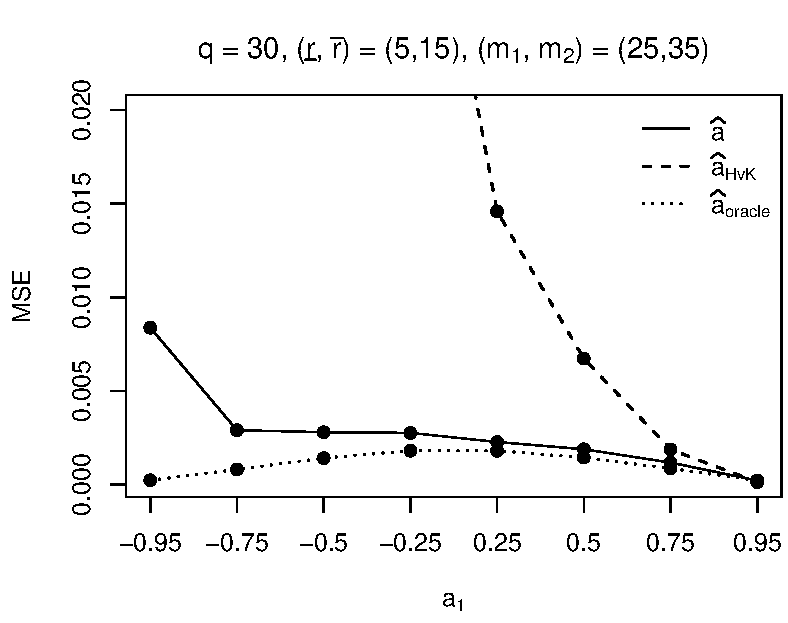
\includegraphics[width=\textwidth]{Plots/Plots_Supplement/MSE_a_zoom_T=500_slope=10_(L1,L2,K1,K2,M1,M2)=(30,30,5,15,25,35).pdf}
\end{subfigure}

\begin{subfigure}[b]{0.45\textwidth}
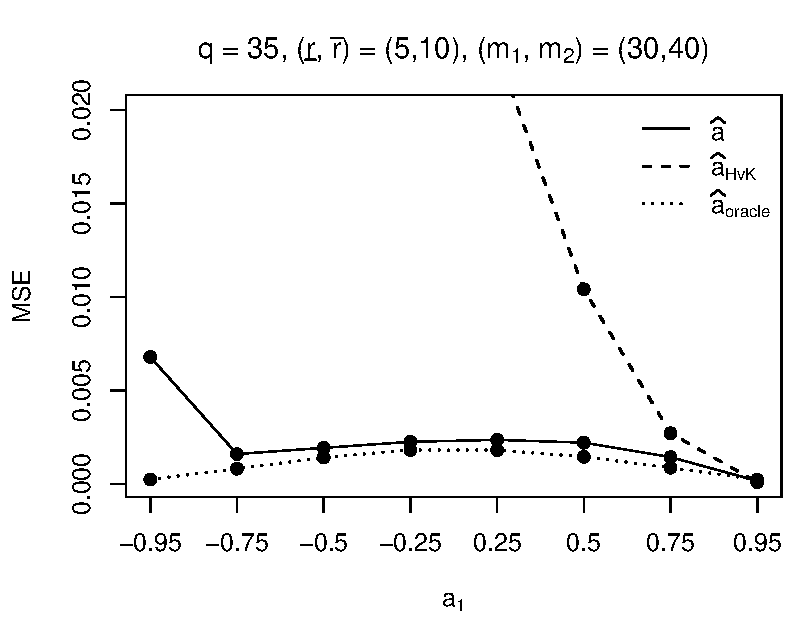
\includegraphics[width=\textwidth]{Plots/Plots_Supplement/MSE_a_zoom_T=500_slope=10_(L1,L2,K1,K2,M1,M2)=(35,35,5,10,30,40).pdf}
\end{subfigure}
\hspace{0.25cm}
\begin{subfigure}[b]{0.45\textwidth}
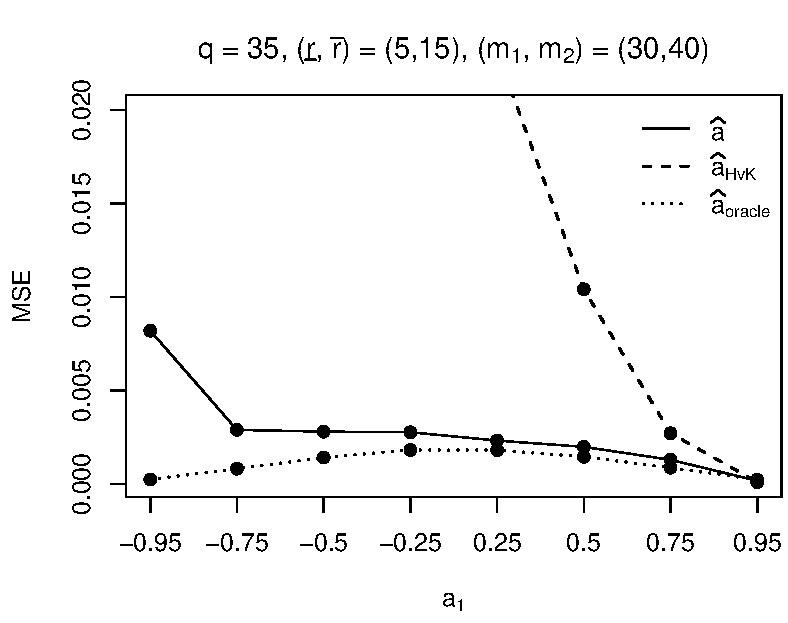
\includegraphics[width=\textwidth]{Plots/Plots_Supplement/MSE_a_zoom_T=500_slope=10_(L1,L2,K1,K2,M1,M2)=(35,35,5,15,30,40).pdf}
\end{subfigure}
\caption{MSE values for the estimators $\widehat{a}$, $\widehat{a}_{\text{HvK}}$ and $\widehat{a}_{\text{oracle}}$ in the scenario with $T=500$ and $s_\beta=10$.}\label{fig:MSE_slope10_AR_zoom_robust} 
\end{figure}


\begin{figure}[p]
\begin{subfigure}[b]{0.45\textwidth}
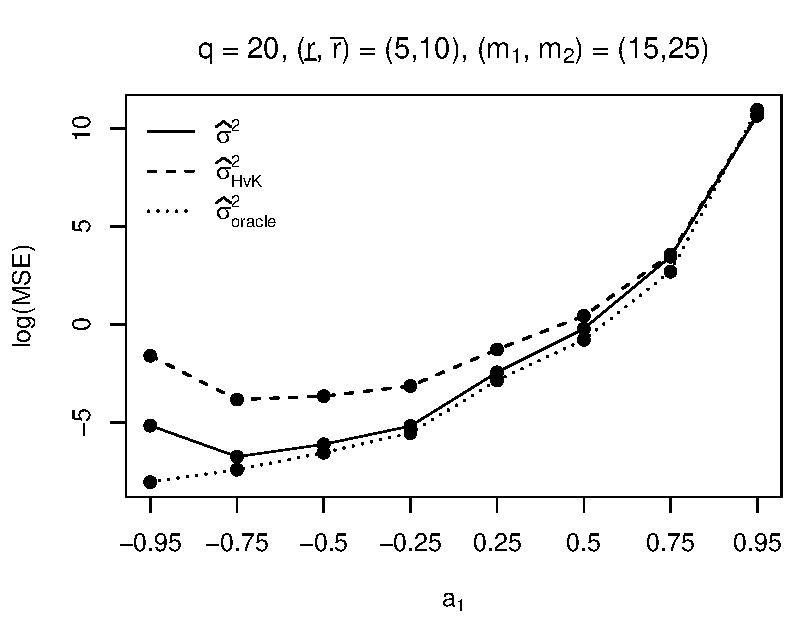
\includegraphics[width=\textwidth]{Plots/Plots_Supplement/MSE_lrv_T=500_slope=10_(L1,L2,K1,K2,M1,M2)=(20,20,5,10,15,25).pdf}
\end{subfigure}
\hspace{0.25cm}
\begin{subfigure}[b]{0.45\textwidth}
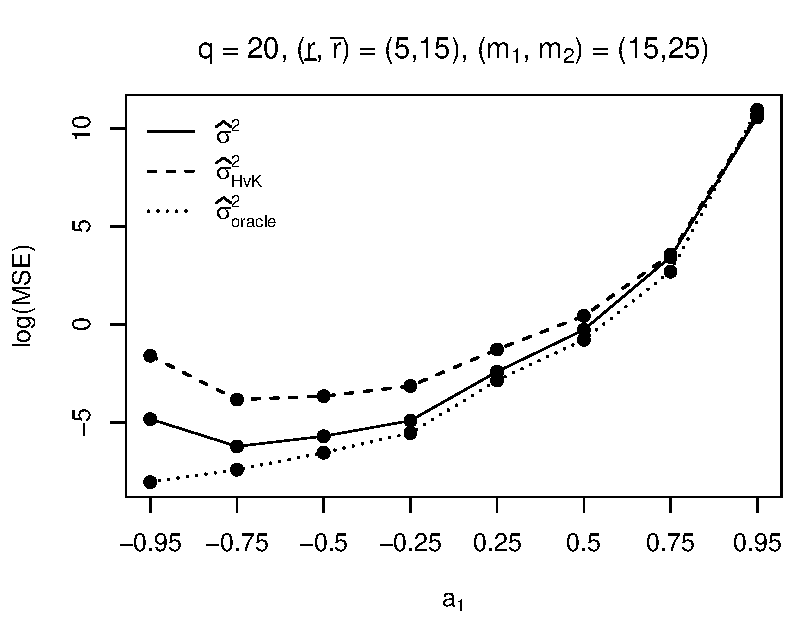
\includegraphics[width=\textwidth]{Plots/Plots_Supplement/MSE_lrv_T=500_slope=10_(L1,L2,K1,K2,M1,M2)=(20,20,5,15,15,25).pdf}
\end{subfigure}

\begin{subfigure}[b]{0.45\textwidth}
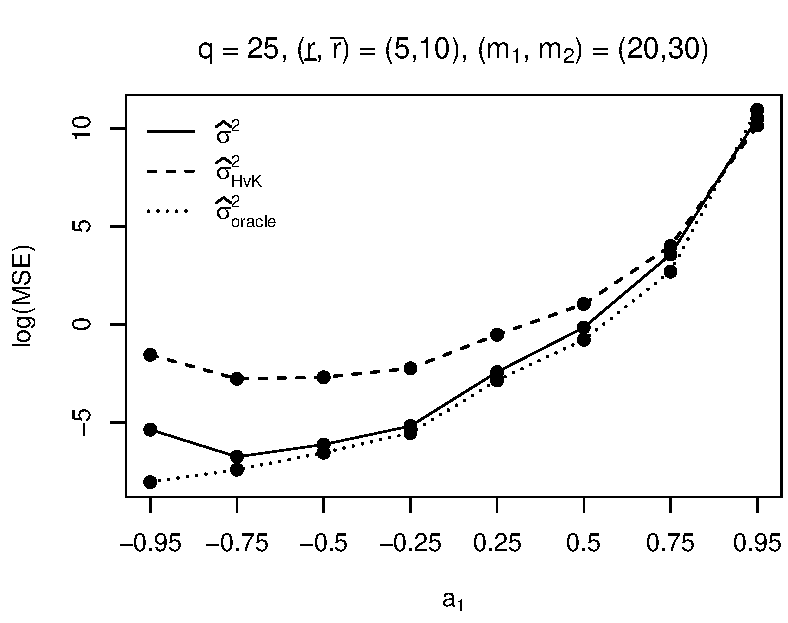
\includegraphics[width=\textwidth]{Plots/Plots_Supplement/MSE_lrv_T=500_slope=10_(L1,L2,K1,K2,M1,M2)=(25,25,5,10,20,30).pdf}
\end{subfigure}
\hspace{0.25cm}
\begin{subfigure}[b]{0.45\textwidth}
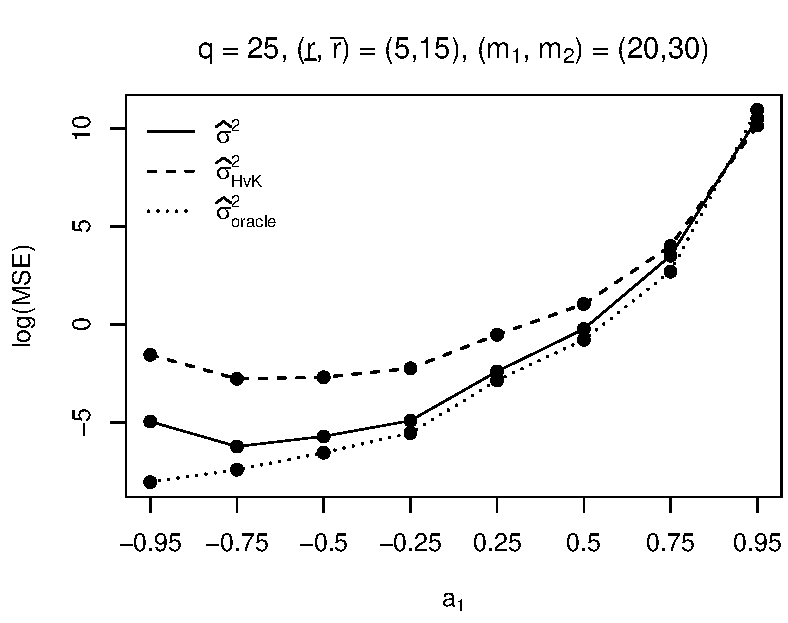
\includegraphics[width=\textwidth]{Plots/Plots_Supplement/MSE_lrv_T=500_slope=10_(L1,L2,K1,K2,M1,M2)=(25,25,5,15,20,30).pdf}
\end{subfigure}

\begin{subfigure}[b]{0.45\textwidth}
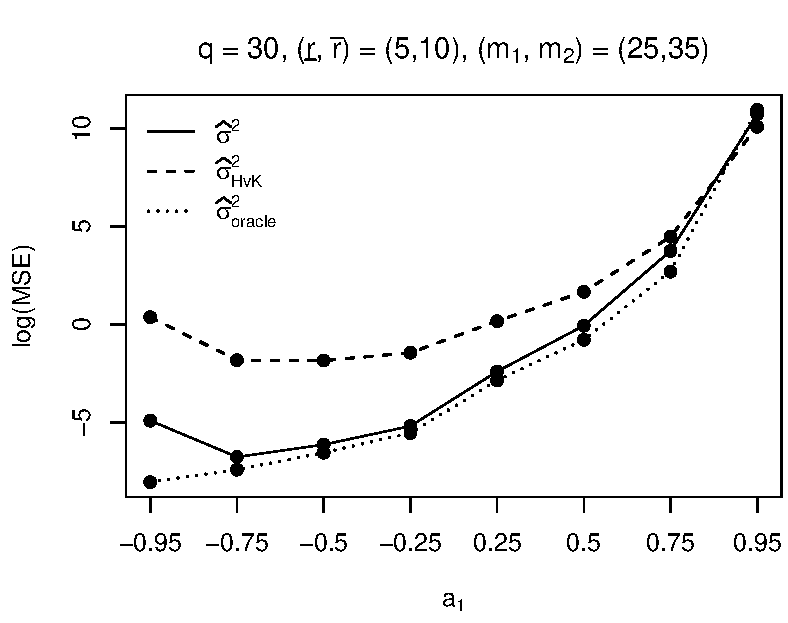
\includegraphics[width=\textwidth]{Plots/Plots_Supplement/MSE_lrv_T=500_slope=10_(L1,L2,K1,K2,M1,M2)=(30,30,5,10,25,35).pdf}
\end{subfigure}
\hspace{0.25cm}
\begin{subfigure}[b]{0.45\textwidth}
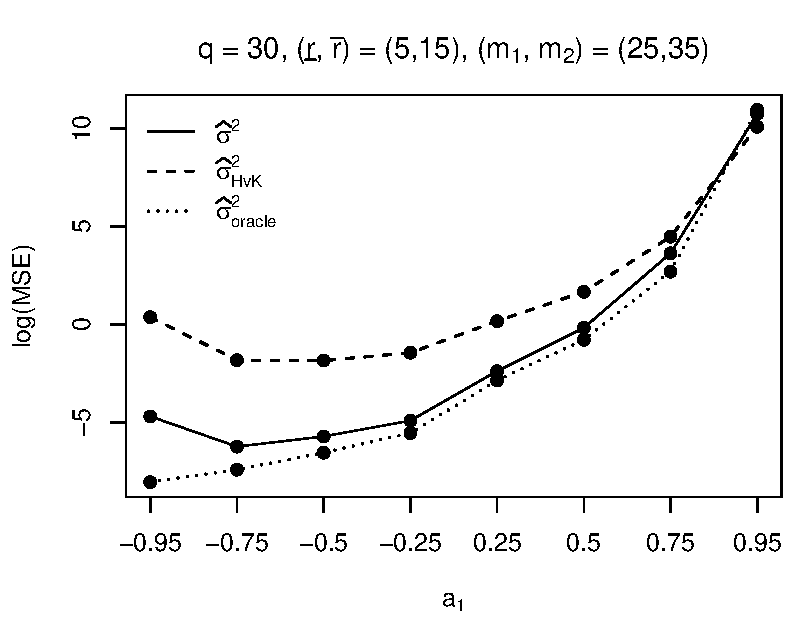
\includegraphics[width=\textwidth]{Plots/Plots_Supplement/MSE_lrv_T=500_slope=10_(L1,L2,K1,K2,M1,M2)=(30,30,5,15,25,35).pdf}
\end{subfigure}

\begin{subfigure}[b]{0.45\textwidth}
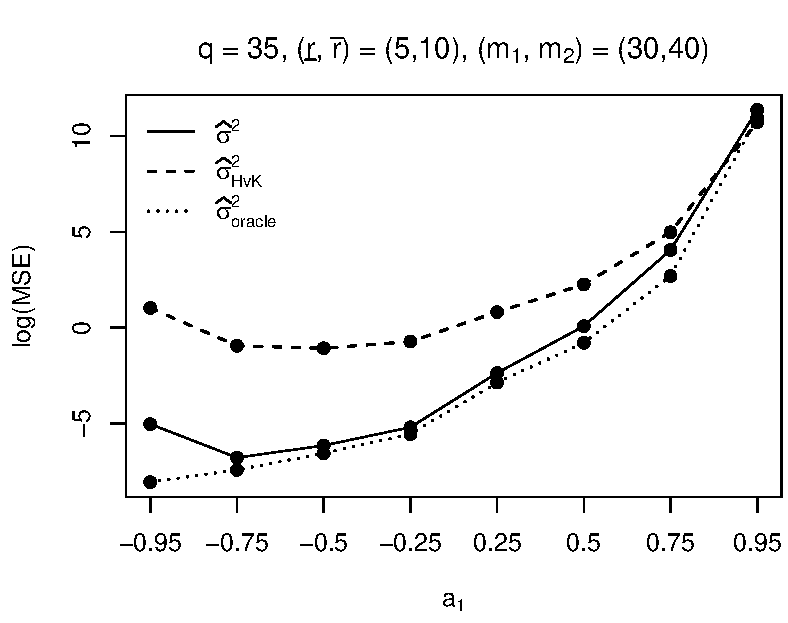
\includegraphics[width=\textwidth]{Plots/Plots_Supplement/MSE_lrv_T=500_slope=10_(L1,L2,K1,K2,M1,M2)=(35,35,5,10,30,40).pdf}
\end{subfigure}
\hspace{0.25cm}
\begin{subfigure}[b]{0.45\textwidth}
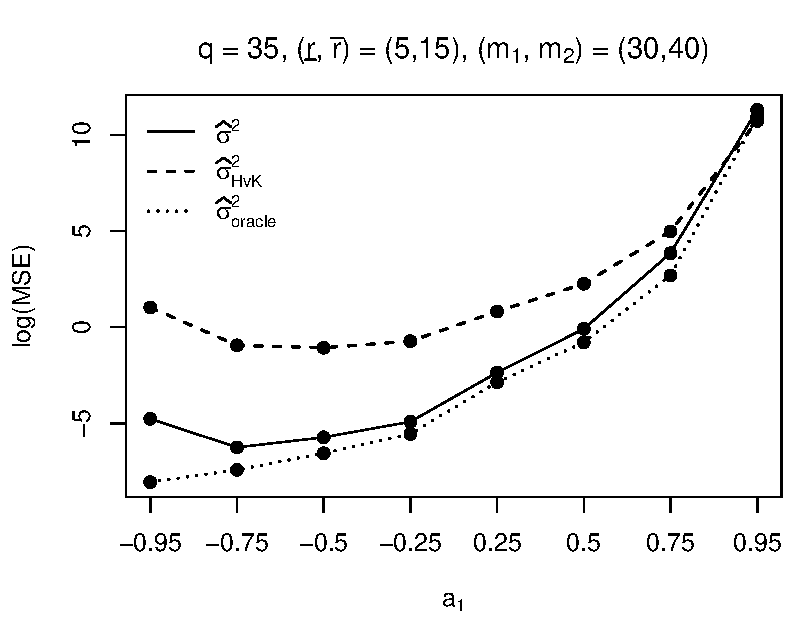
\includegraphics[width=\textwidth]{Plots/Plots_Supplement/MSE_lrv_T=500_slope=10_(L1,L2,K1,K2,M1,M2)=(35,35,5,15,30,40).pdf}
\end{subfigure}
\caption{Logarithmic MSE values for the estimators $\widehat{\sigma}^2$, $\widehat{\sigma}^2_{\text{HvK}}$ and $\widehat{\sigma}^2_{\text{oracle}}$ in the scenario with $T=500$ and $s_\beta=10$.}\label{fig:MSE_slope10_lrv_robust} 
\end{figure}


\subsection*{Implementation of SiZer in Section \ref{subsec-sim-2}}


The SiZer methods for the comparison study in Section \ref{subsec-sim-2} are implemented as follows:
\begin{enumerate}
	\item Calculate $\gamma(k) = \frac{\sigma_\eta^2 }{1 - a_1^2}\cdot a_1^{|k|}$.
	\item Calculate $\var(\bar{Y}) = \frac{\gamma(0)}{T} + \frac{2}{T} \sum_{k = 1}^{T-1} \big(1 - \frac{k}{T}\big)\gamma(k)$.
	\item Calculate $T^* = \frac{\gamma(0)}{\var(\bar{Y})}$.
	\item For each location $i = 1/T, 2/T, \ldots, 1$ and each bandwidth $h = 3/T, 8/T,\ldots, 1/4 + 3/T$ we calculate the following values:
	\begin{itemize}
		\item $ESS(i, h) = \frac{\frac{1}{h}\sum_{t =1}^T K\big(\frac{i - t/T}{h}\big)}{\frac{1}{h}K(0)}$;
		\item $ESS^*(i, h) =\frac{T^*}{T} \cdot ESS$;
		\item $l(i, h) = \frac{T}{ESS^*(i, h)}$;
		\item $q(i, h) = \Phi^{-1} \Big(\frac{1 + (1 - \alpha)^{\frac{1}{l(i, h)}}}{2}\Big)$;
		\item $(X^T W X)^{-1} X^T W$, where $W = \{diag(\frac{1}{h} K\big(\frac{i - t/T}{h}\big))\}$ and 
			\begin{equation}
			X =  \left( \begin{array}{c c}
   					1 & (1/T - i) \\
					1 & (2/T - i)  \\
					\vdots & \vdots \\
					1 & (1 - i)  \\
				   \end{array} \right); \nonumber
			\end{equation}
		\item $sd(\widehat{m}^\prime_h(i)) = \sqrt{\big((X^T W X)^{-1} (X^T \Sigma X) (X^T W X)^{-1}\big)_{2, 2}}$, where $\Sigma$ is the kernel weighted covariance matrix of errors with generic element $$\sigma_{kl} = \gamma(|k - l|) \frac{1}{h} K\Big(\frac{i - k/T}{h}\Big) \frac{1}{h}  K\Big(\frac{i - l/T}{h}\Big).$$
	\end{itemize}
	\item\label{discarding} Discard all pairs of location and bandwidth $(i, h)$ where $ESS^* < 5$.
	\item Based on the grid from \ref{discarding}, calculate Gaussian quantile for our method.
	\item 
\end{enumerate}
